\documentclass[12pt, oneside]{book}  % jednostranna tlac
%\documentclass[12pt, twoside]{book}  % obojstranna tlac

%spravne nastavenie okrajov
\usepackage[a4paper,top=2.5cm,bottom=2.5cm,left=3.5cm,right=2cm]{geometry}
%zapnutie fontov pre UTF8 kodovanie
\usepackage[utf8]{inputenc}
\usepackage[T1]{fontenc}
\usepackage{amsmath}
\usepackage{lipsum}
\usepackage{caption}
\usepackage{booktabs}
\usepackage{subcaption}
\usepackage[section]{placeins}
\usepackage{microtype}
\usepackage{tabularx}    % Pre inteligentné tabuľky a stĺpec typu X
\usepackage{array}       % Pre pokročilé formátovanie stĺpcov (>{\raggedright...})
\usepackage[acronym, nonumberlist]{glossaries}
\makenoidxglossaries
\newacronym{mp}{MP}{Monetary Policy}
\newacronym{mps}{MPS}{Monetary Policy Statement}
\newacronym{nlp}{NLP}{Natural Language Processing}
\newacronym{ecb}{ECB}{European Central Bank}
\newacronym{fed}{FED}{Federal Reserve}
\newacronym{gc}{GC}{Governing Council}
%zapnutie slovenskeho delenia slov
%a automatickych nadpisov ako Obsah, Obrázok a pod. v slovencine
%\usepackage[slovak]{babel} % vypnite pre prace v anglictine!

%nastavenie riadkovania podla smernice
\linespread{1.25} % hodnota 1.25 by mala zodpovedat 1.5 riadkovaniu

% balicek na vkladanie zdrojoveho kodu
\usepackage{listings}
% ukazky kodu su cislovane ako Listing 1,2,...
% tu je Listing zmenene na Algorithm 1,2,...
\renewcommand{\lstlistingname}{Algorithm}
% nastavenia balicka listings
% mozete pridat aj language=...
% na nastavenie najcastejsie pouzivaneho prog. jazyka
% takisto sa da zapnut cislovanie riadkov
\lstset{frame=lines}

% balicek na vkladanie obrazkov
\usepackage{graphicx}
% balicek na vkladanie celych pdf dokumentov, tu zadanie
\usepackage{pdfpages}
% balicek na spravne formatovanie URL
\usepackage{url}
\usepackage{xurl}
\usepackage{tikz}
\usetikzlibrary{shapes.geometric, arrows, positioning} % pridané 'positioning' pre lepšie medzery

% Definícia štýlov
\tikzstyle{startstop} = [rectangle, rounded corners, minimum width=3cm, minimum height=1cm, text centered, draw=black, fill=red!30, align=center]
\tikzstyle{process} = [rectangle, minimum width=3cm, minimum height=1cm, text centered, draw=black, fill=orange!30, align=center]
\tikzstyle{arrow} = [thick,->,>=stealth]
% balicek na hyperlinky v ramci dokumentu
% zrusime farebne ramiky okolo liniek aby pdf
% vyzeralo rovnako ako tlacena verzia
\usepackage[hidelinks,breaklinks]{hyperref}


% -------------------
% --- Definicia zakladnych pojmov
% --- Vyplnte podla vasho zadania, rok ma byt rok odovzdania
% -------------------
\def\mfrok{2026}
\def\mfnazov{Machine Learning Assessment of the Trading Value of Central Bank Information}
\def\mftyp{Bachelor Thesis}
\def\mfautor{Jakub Novotný}
\def\mfskolitel{Ing. Pavel Gertler, PhD. }

%ak mate konzultanta, odkomentujte aj jeho meno na titulnom liste
\def\mfkonzultant{tit. Meno Priezvisko, tit. }  

\def\mfmiesto{Bratislava, \mfrok}

% študenti BIN a DAV odkomentujú príslušnú dvojicu riadkov
% \def\mfodbor{ Computer Science }
% \def\program{ Computer Science }
% pre BIN:
%\def\mfodbor{ Computer Science and Biology }
%\def\program{ Bioinformatics }
% pre DAV:
\def\mfodbor{ Computer Science and Mathematics }
\def\program{ Data Science }

% Uvádzajte pracovisko zo zadania
% u školiteľov z FMFI to bude katedra školiteľa
\def\mfpracovisko{ Department of Computer Science }

\begin{document}     
\frontmatter
\pagestyle{empty}

% -------------------
% --- Obalka ------
% -------------------

\begin{center}
  \sc\large
  Comenius University in Bratislava\\
  Faculty of Mathematics, Physics and Informatics

\vfill

{\LARGE\mfnazov}\\
\mftyp
\end{center}

\vfill

{\sc\large 
\noindent \mfrok\\
\mfautor
}

\cleardoublepage
% --- koniec obalky ----

% -------------------
% --- Titulný list
% -------------------

\noindent

\begin{center}
\sc  
\large
  Comenius University in Bratislava\\
  Faculty of Mathematics, Physics and Informatics

\vfill

{\LARGE\mfnazov}\\
\mftyp
\end{center}

\vfill

\noindent
\begin{tabular}{ll}
Study Programme: & \program \\
Field of Study: & \mfodbor \\
Department: & \mfpracovisko \\
Supervisor: & \mfskolitel \\
% Consultant: & \mfkonzultant \\
\end{tabular}

\vfill


\noindent \mfmiesto\\
\mfautor

\cleardoublepage
% --- Koniec titulnej strany


% -------------------
% --- Zadanie z AIS
% -------------------
% v elektronickej verzii sa zverejňuje zadanie bez podpisov
% v pracach v angličtine anglické aj slovenské zadanie

\newpage
\setcounter{page}{3}
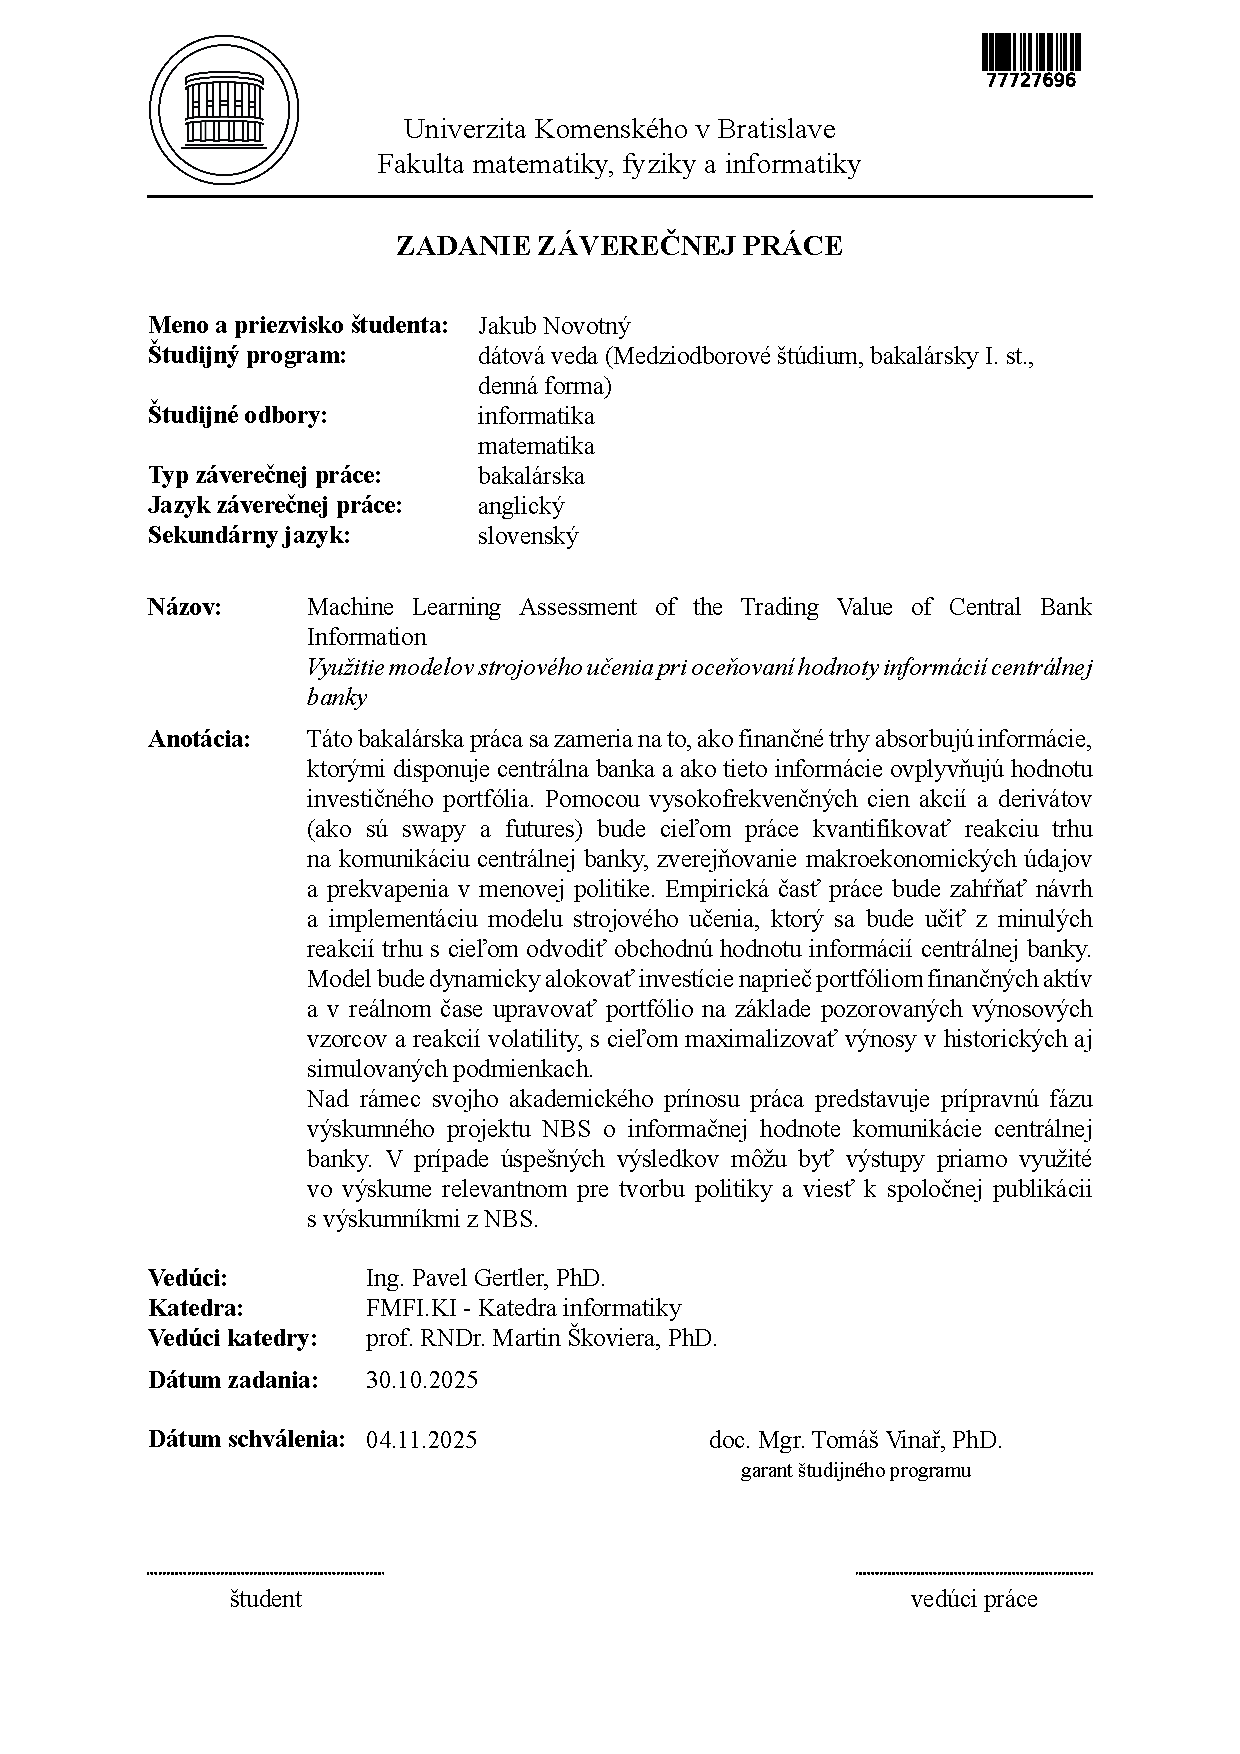
\includepdf{images/zadanie.pdf}

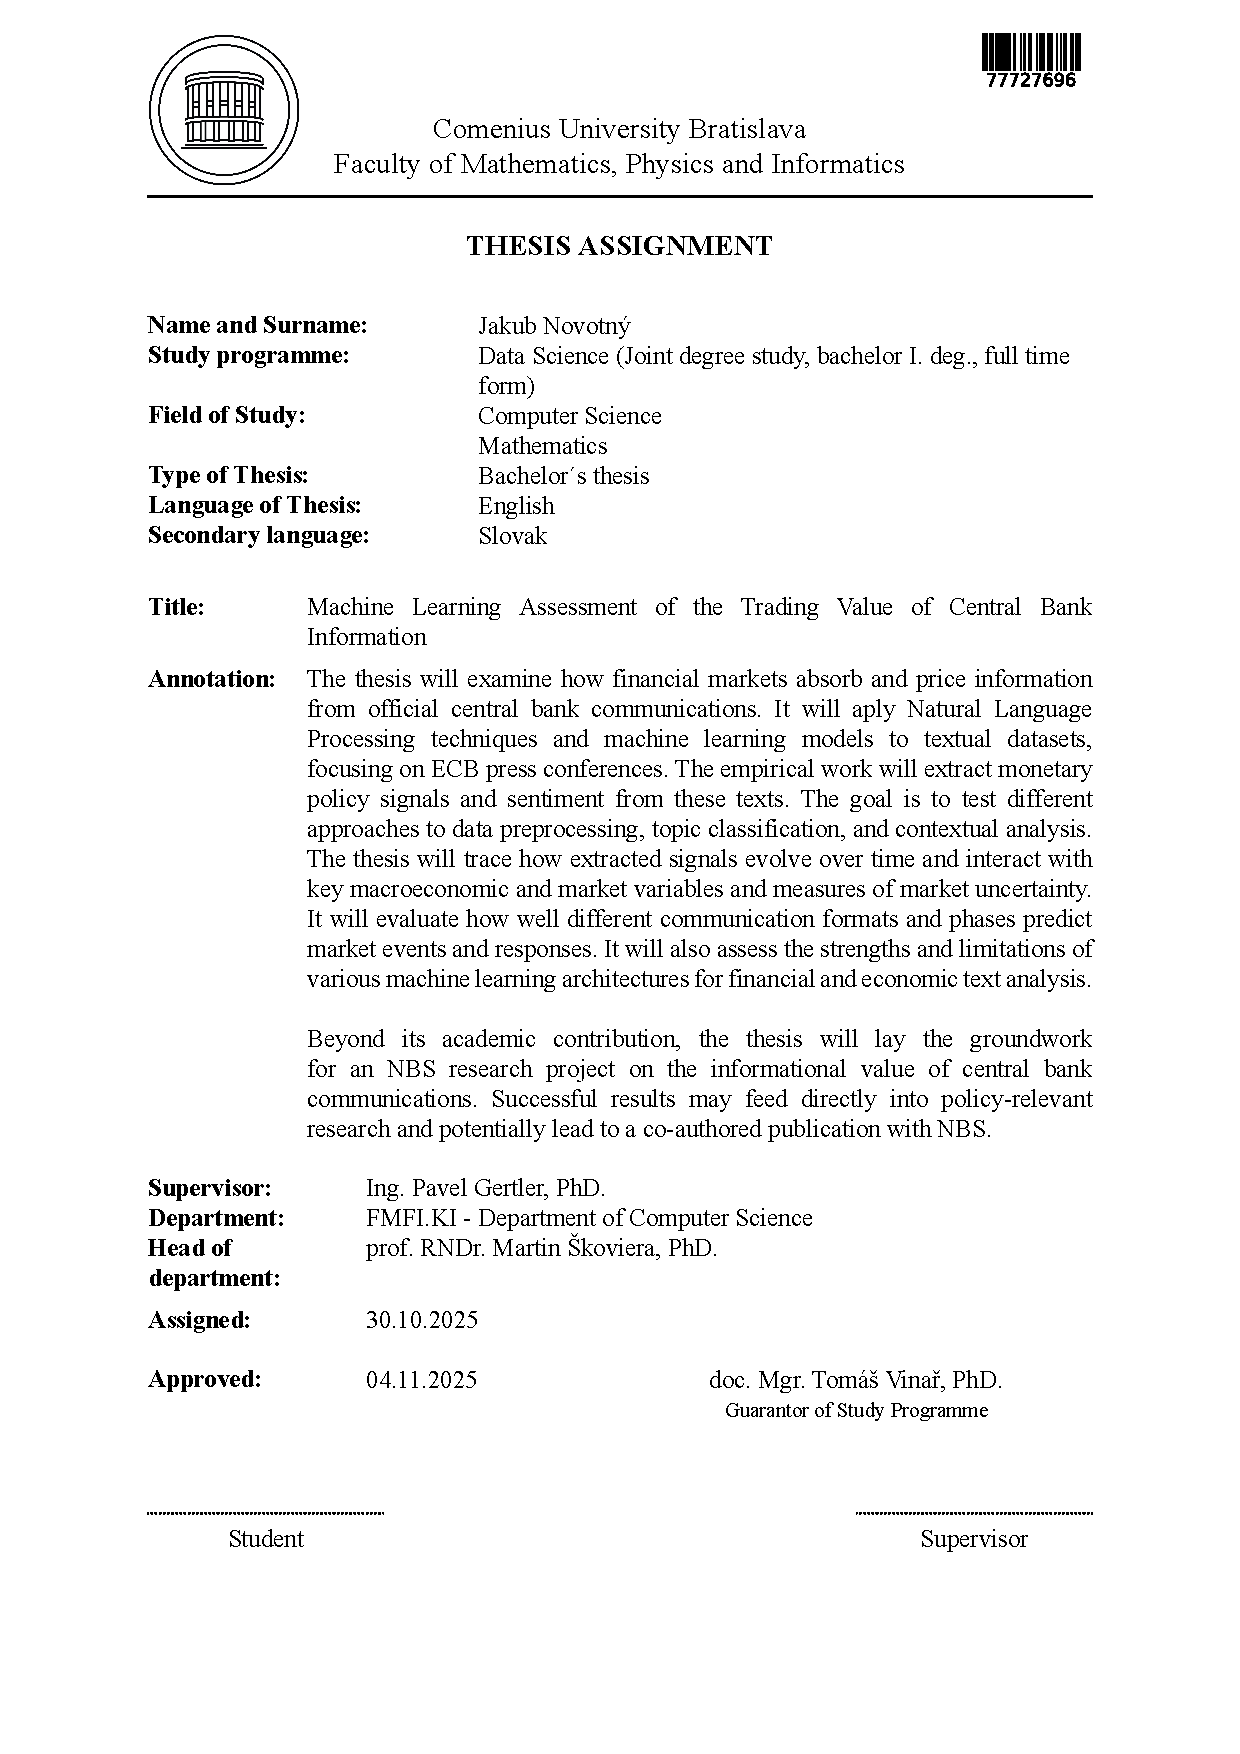
\includepdf{images/zadanie-en.pdf}

% --- Koniec zadania


% -------------------
%   Čestné vyhlásenie a nepovinné poďakovanie
% -------------------
\newpage
\pagestyle{plain}
\paragraph{Declaration:}
I hereby declare that I have independently written this entire bachelor thesis entitled ``\mfnazov'', including all its figures and appendices, using the literature listed in the attached bibliography.

% Uveďte na čo ste nástroje používali
% Podľa typu použitia potom nástroje aj citujte v texte
In preparation of the thesis I have also used the following artifical infelligence tools: Gemini and Claude for the better verbal expression, helping with source searching and writing the Python code for making the plots. I have used artificial intelligence tools in accordance with relevant legal regulations, academic rights and freedoms, ethical and moral principles while simultaneously maintaining academic integrity. I am aware that I am fully responsible for the accuracy of the final text.

\paragraph{Acknowledgments:}
I would like to thank to my supervisor Ing. Pavel Gertler, PhD, for his advice, spent time and interesting conversations about macroconomy. Last but not least, I would like to thank my family, friends and girlfriend for enduring my emotional outbursts, encouraging me and helping me finish my bachelor's degree.

% --- Koniec poďakovania

% -------------------
%   Abstrakt - Slovensky
% -------------------
\newpage 
\section*{Abstrakt}

\paragraph*{Kľúčové slová:} 
analýza sentimentu, tematické modelovanie, menová politika, prediktívna analýza
% --- Koniec Abstrakt - Slovensky


% -------------------
% --- Abstrakt - Anglicky 
% -------------------
\newpage 
\section*{Abstract}

\paragraph*{Keywords:} 
sentiment analysis, topic modeling, monetary policy, predictive analysis

% --- Koniec Abstrakt - Anglicky

% -------------------
% --- Predhovor 
% -------------------
%\newpage 
%
%
%\chapter*{Preface} %
%
%Predhovor je všeobecná informácia o práci, obsahuje hlavnú charakteristiku práce 
%a okolnosti jej vzniku. Autor zdôvodní výber témy, stručne informuje o cieľoch 
%a význame práce, spomenie domáci a zahraničný kontext, komu je práca určená, 
%použité metódy, stav poznania; autor stručne charakterizuje svoj prístup a svoje
%hľadisko. 
%
% --- Koniec Predhovor


% -------------------
% --- Obsah
% -------------------

\cleardoublepage 

\tableofcontents

% ---  Koniec Obsahu

% -------------------
% --- Zoznamy tabuliek, obrázkov, skratiek, slovník - nepovinné
% -------------------

\newpage 

\listoffigures
\listoftables
\printnoidxglossary[type=\acronymtype, title=List of Abbreviations]

% ---  Koniec Zoznamov

\mainmatter
\pagestyle{headings}

\chapter*{Introduction} % chapter* je necislovana kapitola
\addcontentsline{toc}{chapter}{Introduction} % rucne pridanie do obsahu
\markboth{Introduction}{Introduction} % vyriesenie hlaviciek

In this thesis, we will investigate the relationship between central bank communication and financial market reactions, with a specific focus
on the European Central Bank (ECB). %Central banks play a crucial role in shaping economic expectations and influencing financial markets through
%their communication strategies. The ECB, as the central bank for the Eurozone, regularly communicates its monetary policy decisions and economic
%outlook through various channels, including the widely followed Monetary Policy (MP) Statement. This statement, released after each Governing
%Council meeting, provides insights into the ECB's assessment of the economic environment and its future policy intentions.
%
%Understanding the content and tone of these communications is essential for market participants, as they can significantly impact
%asset prices, interest rates, and overall market sentiment. By applying Natural Language Processing (NLP) techniques to analyze the textual content
%of the ECB's MP Statements, we will aim to extract sentiment signals that can be correlated with financial market reactions.
%
%This analysis will contribute to the growing body of research on central bank communication and its implications for financial markets, providing
%insights into how market participants interpret and respond to central bank messaging. The findings of this thesis may have practical implications
%for investors, policymakers, and researchers interested in the dynamics of central bank communication and its influence on financial markets.
\chapter{Theoretical Background}\label{ch:theory}
This chapter establishes the theoretical foundation for the research by connecting the macroeconomic concepts of \gls{mp} with advanced language technology. First, it explores the evolution of central bank communication, emphasising the structural nuances of the \gls{ecb}'s press conferences. Second, it introduces Natural Language Processing as a methodological bridge, tracing the shift from traditional sentiment lexicons to specialised transformer models capable of decoding \gls{ecb} narratives. Finally, the chapter defines the quantitative targets ranging from official policy rates to high-frequency market expectations and structural shocks, providing the framework needed to assess the real-world financial impact of central bank text.

\section{Central Bank Communication}
Over the past three decades, central banking has undergone fundamental changes in its disclosure structures. Before the 1990s, there was no public explanation of why monetary policy decisions were made. Policymakers believed that a degree of unpredictability enhanced the effectiveness of policy interventions. This period of institutional unpredictability was characterised by a marked lack of formal public guidance \cite[p. 3]{NBERw11898}. Market participants repeatedly had to guess the target interest rate and the bank's policy setting. They relied on the size, timing, and nature of the operations conducted by the \gls{fed} trading departments in the open market.

Since then, communication has evolved from a peripheral public relations function to a core instrument of \gls{mp}. Central banks have increasingly recognised transparency and accountability as fundamental public service obligations \cite[p. 15--18]{blinder2008central}. Beyond institutional accountability, the evolution of \gls{mp} frameworks has demonstrated that transparent and credible central banks are considered important for maintaining long-term price stability \cite{daly2025dynamic}. This is particularly evident in the widespread adoption of inflation targeting across advanced and emerging economies. Empirically, clear communication has been shown to enhance central bank independence, strengthen institutional credibility, and anchor inflation expectations in complex macroeconomic environments \cite[p. 7]{filardo2008transparency}.

\paragraph{The European Central Bank Framework}
Within the Eurozone, the \gls{ecb} faces a communication challenge: it must address a fragmented, multi-national audience while maintaining a unified monetary stance. Since its establishment in 1999, the \gls{ecb}'s communication framework has progressively evolved to anchor expectations across diverse sovereign bond markets. This institutional evolution is most evident in its structured approach to policy announcements \cite{ECB_about}.

\subsection{Monetary Policy Statement}
\label{subsection:mps}
At the operational core of the \gls{ecb}'s communication strategy is the \gls{mps}, which is delivered during the press conference that directly follows the \gls{mp} meetings of the \gls{gc}. The council consists of the six members of the Executive Board (including the President and Vice-President) and the governors of the euro area national central banks, who meet to deliberate and set monetary policy parameters for the entire currency bloc. The \gls{ecb} currently schedules eight \gls{mp} meetings per year, operating on an approximate six-week cycle \cite{ITC_ECB_Schedule}.

\paragraph{Schedule of the Governing Council Meeting Day}
The organisation of the announcement day is standardised, reflecting the institution's strict commitment to predictability and the mitigation of market volatility. Starting from July 21, 2022, the \gls{ecb} modified its historical publication timeline to optimise the way financial markets process complex policy signals \cite{ECB2022_NewTimes}. The initial policy decision---usually a short press release detailing the exact interest rate parameters, deposit facility rates, and main structural changes to asset purchase programmes---is published at 14:15 CET. Shortly afterward, the press conference begins at 14:45 CET, during which the \gls{ecb} President and Vice-President present the detailed \gls{mps} and interact directly with the financial press. In parallel with the start of the \gls{qa} segment, the full text of the \gls{mps} is published on the \gls{ecb}'s digital platforms at 15:00 CET. At 17:00, European stock markets close independently of the \gls{ecb}, ending the day's reactions to its actions, as shown in Table~\ref{tab:meet_schedule}.

\begin{table}[ht]
    \centering
    \caption[Governing Council Meeting Day Schedule]{Governing Council Meeting Day Schedule.}
    \label{tab:meet_schedule}
    \begin{tabular}{@{}lr@{}}
        \toprule
        \textbf{Event}                         & \textbf{Scheduled time (CET)} \\ \midrule
        Meeting of the \gls{gc}                & 9:00 -- 12:00                 \\
        \gls{mp} announcement                  & 14:15                         \\
        Press conference (IS + \gls{qa}) & 14:45 -- 15:15                \\
        European stock market close            & 17:00                         \\ \bottomrule
    \end{tabular}
\end{table}


\paragraph{Structure of the Press Conference}
\label{sec:press_structure}
The press conference itself is divided into two distinct communication phases: the reading of the formally prepared \gls{is} and the subsequent unscripted \gls{qa} session. This structural division is not merely procedural; it has measurable consequences for financial markets, as the two sections serve different informational functions and generate distinct asset price dynamics.

The \gls{is} is a structured, carefully drafted document that represents the \gls{gc}'s consensus view \cite{ECB_WP2742}. It provides a linear overview of the economic assessment, inflation dynamics, and the evaluation of monetary and financial conditions. The language used in this document is deliberately precise, relying on specific syntactical formulations to signal the future policy path. This practice is commonly known as forward guidance: an explicit communication tool by which the central bank provides forward-looking indications about the future trajectory of its policy rates or asset purchases, thereby shaping market expectations beyond the current meeting \cite{blinder2008central}.

In contrast, the \gls{qa} session introduces a semi-structured interaction. Advanced textual analysis and structural topic modelling of historical transcripts demonstrate that the thematic content of the statement differs from the discourse during the \gls{qa} session. The topics dominating the statement are persistent, structural, and strongly focused on standardised macroeconomic aggregates. Conversely, the \gls{qa} often introduces new topics that were not addressed in the prepared text. Empirical research reveals that the first six most prevalent topics within a vast sample of press conference transcripts are predominantly driven by the \gls{qa} segments. This suggests that a significant share of the added value of the press conference lies in the \gls{qa} phase, which provides the public and market participants with detailed explanations regarding the \gls{ecb}'s decisions in real time \cite{ECB_WP2742}.

\subsection{Other Communication Channels}
While the \gls{mps} and the accompanying press conference represent the focal point of the \gls{ecb}'s communication strategy, they are complemented by a broader set of publications, reports, and public engagements. To continuously influence the yield curve, anchor long-term expectations, and fulfill its mandate of transparency, the \gls{ecb} applies several supplementary communication channels in the weeks between formal \gls{gc} meetings. This \emph{inter-meeting communication} is an effective mechanism for managing expectations between meetings and for addressing structural complexities and the mechanics of financial transmission. These details cannot be fully addressed in a single monthly press conference \cite{Istrefi2021ECB}.

\paragraph{The Economic Bulletin} is a comprehensive analytical publication that explains the reasons behind the \gls{mp} decisions of the \gls{ecb}'s Governing Council. Published eight times a year---generally two weeks after the corresponding \gls{mp} meeting---the Bulletin contextualises the Governing Council's decisions against the detailed backdrop of prevailing economic, financial, and monetary conditions \cite{press_to_speeches}.

\paragraph{The Monetary Policy Accounts} represent a significant transparency reform. The \gls{ecb} began publishing regular accounts of the Governing Council's \gls{mp} meetings in early 2015, aligning its institutional practices with those of the US \gls{fed} and the Bank of England. These accounts are typically released four weeks after the corresponding meeting \cite{MP_accounts}.

The documents offer a detailed overview of the Governing Council's internal deliberations. They outline the delicate balance of arguments, the range of risk assessments considered by various members, and the different perspectives on the economic outlook. By documenting the full range of analytical debates, the accounts help market participants understand the central bank's internal response function and the specific macroeconomic thresholds that might trigger future policy interventions \cite[p. 26--27]{CorbisieroLawton2021}.

As the \gls{ecb}'s communication channels have multiplied to foster transparency, the volume of textual data generated by the central bank has expanded substantially. While human analysts can interpret individual statements, the sheer scale and frequency of this qualitative information necessitate computational approaches to systematically extract the monetary policy signals. This demand for automated, large-scale text analysis motivates the application of \gls{nlp}.

\section{Natural Language Processing in Finance}
The growing availability of digital information has transformed the methodology of financial and macroeconomic research. Historically, empirical finance has relied almost exclusively on structured, quantitative data. However, language has always shaped financial markets, and unstructured textual data---ranging from earnings call transcripts to central bank \gls{mps}---contains critical information about the future. \gls{nlp} serves as a technological linkage, enabling researchers and practitioners to systematically extract structured, machine-readable signals from these vast corpora of unstructured text \cite{IBM_IE_2025}. In the context of \gls{mp}, \gls{nlp} algorithms are used to quantify the qualitative narratives of central bankers, capturing nuances in market psychology and institutional sentiment.

\subsection{Concept of Sentiment Analysis}
\label{sec:sentiment_concept}
Sentiment analysis is the computational extraction of subjective information and emotional states from text, with the central task of classifying a passage's underlying \textit{polarity} \cite{xing2020financial}. In its canonical formulation the polarity is mapped onto a positive--neutral--negative axis, where \textit{positive} denotes affirmative or optimistic framing and \textit{negative} denotes adverse or pessimistic framing.

Early applications in finance relied on dictionary-based approaches, which measure sentiment by aggregating the frequency of predefined terms. A common metric in this tradition is a normalised difference between positive and negative word counts. However, as noted by Loughran and McDonald \cite{LoughranMcDonald2011}, standard baseline dictionaries routinely misclassify common financial terminology; the word \textit{liability}, for example, is negative in general parlance but serves as a neutral, descriptive accounting term in financial filings. This mismatch motivated the development of domain-specific lexicons to accurately measure sentiment in corporate and macroeconomic contexts \cite{LoughranMcDonald2011}.

As deep learning matured, the methodology of sentiment quantification has shifted from counting isolated words to processing contextual probabilities. To facilitate econometric analysis, researchers transform these discrete class probabilities into a continuous \textit{Sentiment Score} ($S$). While the technology has evolved, the logic of aggregation remains similar to classic sentiment indices \cite{gentzkow2019text}. As defined in Equation~\ref{eq:sentiment}, the score is calculated as the difference between the probability assigned to the positive (or hawkish) class and its negative (or dovish) counterpart:

\begin{equation}
    \label{eq:sentiment}
    Score \;=\; P_{\text{positive}} \;-\; P_{\text{negative}},
\end{equation}

where $P \in [0, 1]$ represents the softmax probability assigned by the model to each respective label. This transformation maps the model's probabilistic output onto a linear scale bounded by $-1$ and $+1$. A value of zero signifies either a balanced or a neutrally classified passage. The two classifiers used in this thesis (introduced below) emit a binary positive/negative softmax: passages that the model assigns to a third \textit{neutral} class contribute zero by construction, attenuating the aggregate signal toward zero when a press conference consists predominantly of procedural or descriptive language.

The transition from static lexicons to transformer-based architectures, such as \textsc{bert} (Bidirectional Encoder Representations from Transformers), addresses the inability of bag-of-words models to capture context-dependent relationships. Unlike methods that process words in isolation, \textsc{bert} evaluates each token in relation to all others in a sentence, allowing for a nuanced treatment of syntax, negation, and complex economic narratives.

However, the linguistic requirements of central bank analysis nevertheless necessitate further specialisation. General-purpose models trained on Wikipedia or common literature struggle with the technical and coded lexicon used by monetary authorities \cite{BIS_WP1215_2024}. This limitation motivated the development of domain-adapted sentiment classifiers, of which two are employed in the present work. \textbf{FinBERT} \cite{araci2019finbert} is a BERT-base model further pre-trained on Reuters' TRC2 financial-news corpus and fine-tuned for sentiment on the Financial PhraseBank, and it represents the standard for general financial sentiment. \textbf{CentralBankRoBERTa} \cite{Pfeifer2023} is fine-tuned by Pfeifer and Marohl on a corpus of central bank speeches and reports and represents a further narrowing of the training distribution toward the institutional vocabulary of monetary authorities. Both models output a binary positive/negative polarity in the sense of Equation~\ref{eq:sentiment}; they differ in the domain of their pre-training corpus, not in their classification objective. Their differences are summarised in Table~\ref{tab:model_comparison}.

\begin{table}[ht]
    \centering
    \caption{Evolution of NLP models in financial and central bank contexts.}
    \label{tab:model_comparison}
    \begin{tabular}{@{}lll@{}}
        \toprule
        \textbf{Model} & \textbf{Training Corpus}                 & \textbf{Linguistic Nuance}  \\ \midrule
        BERT           & General (Wikipedia, BookCorpus)          & High (general context)      \\
        FinBERT        & Reuters TRC2 + Financial PhraseBank      & Domain-specific (financial) \\
        CBRoBERTa      & \gls{ecb}/\gls{fed} speeches and reports & Policy-specific (monetary)  \\ \bottomrule
    \end{tabular}
\end{table}

A conceptually distinct strand of the literature seeks to classify not the \emph{emotional} tone of central bank communications but their \emph{policy stance}: whether a passage signals a tightening (``hawkish''), an easing (``dovish'') or no change (``neutral'') in the monetary stance. Stance classification differs from sentiment analysis along two dimensions. First, its label space is operational rather than affective: a sentence such as \textit{``inflation is far too high''} carries a strongly negative emotional tone yet implies a hawkish policy stance, because elevated inflation is the standard precondition for tighter policy. Second, the construction of stance training sets requires manual annotation by domain experts using documented annotation guides, since the mapping from text to policy implication is not recoverable from sentiment cues alone. State-of-the-art stance classifiers for central bank discourse include the FOMC-trained RoBERTa-large model of Shah et al.\ \cite{shah2023trillion} and the multi-bank extension of Shah, Sukhani, Pardawala et al.\ \cite{shah2025wcb}, the latter of which provides a model fine-tuned specifically on \gls{ecb} communications.

These models are released under gated access on the Hugging Face Hub. As access could not be obtained within the timeframe of this study, the present analysis is restricted to sentiment classifiers, and the resulting signal should be interpreted as a measure of the \emph{affective tone} of \gls{ecb} discourse rather than its policy stance. Extending the pipeline to incorporate the stance dimension is identified in Chapter~\ref{ch:discussion} as a priority for future work.

\subsection{Zero-Shot Classification and the NLI Mechanism}
\label{sec:nlp_finance}
While the polarity score provides a measure of the tone of the discourse, it does not identify the subject of that tone. A hawkish signal regarding inflation has vastly different market implications than a hawkish remark regarding structural reforms. Sentiment analysis is therefore often complemented by thematic categorisation.

Traditionally, the thematic analysis of central bank communication was dominated by probabilistic generative models, most notably Latent Dirichlet Allocation (LDA) \cite{blei2003latent}. While useful for broad explorations, these ``bag-of-words'' approaches suffer from significant limitations, specifically an inability to capture semantic context and the requirement for users to pre-specify a fixed number of topics without a deeper understanding of linguistic nuance. To overcome these limitations, the field of financial NLP has increasingly shifted toward neural architectures using transformers and Natural Language Inference (NLI) frameworks \cite{yin2019benchmarking}.

This architectural shift enables \textit{zero-shot classification}: the technique allows a model to categorise text into user-defined labels without any task-specific supervised training. The procedure recasts classification as a logical relationship between a \textit{premise} (the original central bank passage) and a \textit{hypothesis} (a template representing the candidate label, such as \textit{``This passage discusses monetary policy.''}) \cite{yin2019benchmarking}.

To derive a confidence score for a specific category, the model's raw output logits for logical entailment and contradiction are processed through a softmax to yield the probability $P(c_i)$ for each candidate label $c_i$. In the implementation adopted in this work, the BART-large architecture pre-trained on the MultiNLI corpus \cite{lewis2019bart} provides the entailment backbone, and the neutral logit is discarded prior to normalisation:

\begin{equation}
    P(c_i) = \frac{\exp({l_{entail}})}{\exp({l_{entail}}) + \exp({l_{contra}})},
\end{equation}

where $l_{entail}$ and $l_{contra}$ represent the model's raw logits for entailment and contradiction, respectively. This mathematical framework allows the resulting thematic weight to reflect the relative strength of the logical link between the bank's statement and the defined hypothesis.

By combining domain-specific sentiment extraction with zero-shot thematic classification, the qualitative narratives of central bankers are transformed into structured, time-series data. However, to evaluate whether these linguistic signals actually influence financial markets, they must be benchmarked against observable economic variables. This requires an econometric framework capable of quantifying both the official policy stance and the high-frequency market reactions.

\section{Measuring Monetary Policy}
To fill the gap between qualitative NLP outputs and econometric modelling, it is essential to define the quantitative metrics that represent the monetary policy stance and market expectations. This section details the primary indicators used as targets for predictive modelling, ranging from official policy rates to structural market shocks. Table~\ref{tab:mp_indicators} summarises the four indicators that recur throughout the empirical chapters.

\paragraph{Official Policy Rates and the Shadow Rate}
The primary instrument of the \gls{ecb}'s monetary policy is the \gls{mro} rate, which sets the cost of liquidity for the banking system. While the \gls{mro} rate is the explicit signal of the policy stance, its effectiveness as a continuous variable is limited when interest rates reach the \gls{zlb}.

To measure the stance when nominal rates are constrained, researchers employ the \emph{Shadow Rate}. As proposed by \cite{krippner2013measuring} and operationalised for the euro area by Wu and Xia \cite{wu2016measuring}, the shadow rate is a model-based construct that translates unconventional policy measures, such as large-scale asset purchases and forward guidance, into a single interest rate equivalent. Unlike the \gls{mro}, the shadow rate can move into negative territory, providing a more granular metric of monetary conditions during periods of intensive central bank intervention.

\paragraph{Market Expectations and OIS Volatility}
Real-time market reactions to central bank communication are primarily captured using \gls{ois}. An \gls{ois} is a financial derivative where a fixed interest rate is exchanged for a floating overnight rate (specifically the  €STR in the Eurozone) over the duration of the contract. Since there is no exchange of principal and the floating leg is based on an overnight rate, \gls{ois} rates are considered a ``risk-free'' proxy for the market's expectation of the future path of monetary policy.

In the context of the \emph{EA-MPD} dataset \cite{altavilla2019measuring}, the focus is on the \emph{change} in these rates ($\Delta \text{OIS}$) during the press conference window. The dataset provides a term structure of expectations ranging from one month to ten years. Each segment serves a distinct analytical purpose: the short end (1M to 6M) reflects expectations regarding near-term policy rates, the mid-curve (1Y to 2Y) captures the effectiveness of forward guidance, and the long end (5Y to 10Y) acts as a gauge for long-term inflation anchoring.

Beyond the directional shifts in rates, their intraday volatility during the announcement serves as a critical proxy for market uncertainty. A divergence between the \gls{is} and the spontaneous \gls{qa} session---often referred to as a ``communication mismatch''---typically manifests as heightened volatility. This indicates that the market is struggling to price in conflicting signals, making uncertainty a quantifiable dimension of the central bank's communication effectiveness.

\begin{table}[ht]
    \centering
    \caption{Key Monetary Policy Indicators used as empirical targets.}
    \label{tab:mp_indicators}
    \begin{tabular}{@{}ll@{}}
        \toprule
        \textbf{Indicator}        & \textbf{Economic Significance}                                        \\ \midrule
        \gls{mro} Rate            & Direct policy signal and cost of liquidity.                           \\
        Shadow Rate               & Policy stance proxy in \gls{zlb} environments \cite{wu2016measuring}. \\
        \gls{ois} Rates (1M--10Y) & Forward-looking expectations across the yield curve.                  \\
        $PC1$ (Shocks)            & Aggregated policy surprise \cite{jarocinski2020deconstructing}.       \\ \bottomrule
    \end{tabular}
\end{table}

\paragraph{Structural Shocks and Principal Component Analysis}
The ``pure'' impact of a policy announcement is often clouded by the information effect, where markets react to the central bank's economic outlook rather than the policy change itself. To isolate the intended policy signal, \cite{jarocinski2020deconstructing} and \cite{altavilla2019measuring} utilise structural decomposition. By observing the co-movement of interest rates and stock prices, researchers separate these shocks into ``pure monetary'' and ``information'' components. To simplify the multi-dimensional nature of interest rate moves across the yield curve, Principal Component Analysis (PCA) is applied to the high-frequency $\Delta \text{OIS}$ vector. The First Principal Component ($PC1$) is extracted to represent the overarching shift in expectations, as shown in Equation~\ref{eq:pc1}:

\begin{equation}
    \label{eq:pc1}
    PC1_t = \sum_{j=1}^{n} \omega_j \cdot \text{Shock}_{j,t},
\end{equation}

where $\omega_j$ represents the PCA loading for the structural shock at maturity $j$. This $PC1$ serves as a robust target variable for the machine-learning models of Chapter~\ref{ch:results}, as it captures the dominant policy surprise while filtering out idiosyncratic noise from individual maturities.

\paragraph{Chapter Synthesis}
The institutional structure of central bank communication, the computational extraction of sentiment via \gls{nlp}, and the quantitative measurement of monetary policy shocks form the basis of this thesis. By mapping the qualitative shifts in the \gls{ecb}'s discourse onto the structural changes in the \gls{ois} yield curve, the methodology of Chapter~\ref{ch:data} details the empirical framework used to isolate the trading value of monetary policy signals, and the empirical findings of Chapter~\ref{ch:results} evaluate it against the financial-market benchmarks defined above.
\chapter{Data and Methodology}
This chapter outlines the~data collection framework and the~implementation of \gls{nlp} and machine learning model. The~data pipeline begins with the~automated scraping and text processing of the~\gls{ecb}'s monetary policy statement transcripts. The~extracted and processed text is located into a~custom \textit{SQLite} database. In this database we include sentiment and topic metadata, which are formed by \textit{BERT} familiar models and zero-shot topic classifier. This architecture ensures data integrity and provides a~robust foundation for subsequent macroeconomic and market variables interaction modeling.

\section{Data Scraping and Preprocessing}
Datasets of \gls{ecb} communications are publicly available. Nonetheless, for fine-grained sentiment analysis, they lack the~neccessary level of detail. Moreover, most sources provide uniform text blocks without distinguishing between the~\gls{is} and \gls{qa} components. Our decision to develop a~custom scraping pipeline was driven by the~need to isolate the~responses of \gls{ecb} officials from the~questions posed by journalists. This allowed for a~more precise extraction of \gls{mp} signals, which are free from the~sentiment bias caused by journalistic questioning. The~first phase focuses on the~preparation of a~dataset of transcripts from \gls{gc} conferences. This preparation is divided into two primary tasks. The~first task involves the~retrieval of hyperlinks to scrape webpages, while the~second focuses on parsing the~content into two logical segments and storing these parts in a~robust, structured format.

The~scraping pipeline initially retrieves the~raw \textit{HTML} pages and extracts the~relevant textual content. To accurately separate the~\gls{is} from the~\gls{qa} session, the~pipeline utilizes custom Regular Expressions (Regex). After initial investigation, we defined specific structural markers in the~transcripts the~algorithm precisely splits the~document. These markers included phrases such as \textbf{``My first question...''} or \textbf{``Transcript of the~questions''}. Furthermore, within the~\gls{qa} segments, the~script distinguishes the~responses of \gls{ecb} officials from the~journalists' questions. The~raw extracted data, including dates and URLs, are temporarily stored in a~Pipe-Separated Values (.psv) format.

% Samotný diagram
\begin{figure}[ht]
    \centering
    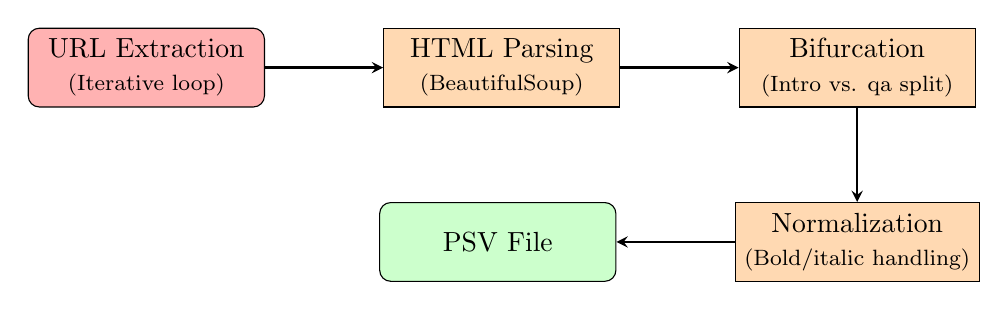
\begin{tikzpicture}[node distance=1.2cm and 1.5cm] % Vertikálna a~horizontálna medzera

        % Prvé tri idú doprava
        \node (start) [startstop] {URL Extraction \\ \footnotesize (Iterative loop)};
        \node (parse) [process, right=of start] {HTML Parsing \\ \footnotesize (BeautifulSoup)};
        \node (bifurc) [process, right=of parse] {Bifurcation \\ \footnotesize (Intro vs. \gls{qa} split)};

        % Štvrtý ide DOLE pod tretí
        \node (norm) [process, below=of bifurc] {Normalization \\ \footnotesize (Bold/italic handling)};

        % Piaty ide DOĽAVA od štvrtého (pod druhý)
        \node (stop) [startstop, left=of norm, fill=green!20] {PSV File};

        % Prepojenia (Arrows)
        \draw [arrow] (start) -- (parse);
        \draw [arrow] (parse) -- (bifurc);
        \draw [arrow] (bifurc) -- (norm);
        \draw [arrow] (norm) -- (stop);

    \end{tikzpicture}
    \caption{The~Data Acquisition and Preprocessing Pipeline}
    \label{fig:data_pipeline_snake}
\end{figure}

\subsection{Iterative Extraction of ECB Discourse}

Before the~text extraction from the~transcript of the~press conference, the~acquisition of the~hyperlink list was required. The~entire acquisition pipeline is visualized in Figure \ref{fig:data_pipeline_snake}. To acquire a~complete list of meeting URLs, the~\textit{HTML} source of the~official \href{https://www.ecb.europa.eu/press/press_conference/monetary-policy-statement/html/index.en.html}{ECB monetary policy statement list} was analyzed. The~primary index page is interactive and necessitates scrolling to load every hyperlink. Therefore, we needed the~implementation of a~\textit{Selenium WebDriver} for browser automation. However, we discovered a~more algorithmically efficient alternative. We managed to retrieve the~backend structure with year-specific placeholders: \nolinkurl{https:// www.ecb.europa.eu/press/press\_conference/monetary-policy-statement/{year}/ html/index\_include.en.html}.

Hence, we applied the~iterative loop across all relevant years. This streamlines the~hypertext link extraction process by avoiding browser interactions. This process, spanning from the~\gls{ecb}'s establishment to the~present, yielded a~total of $291$ unique transcripts.

\subsection{Content Parsing and Data Structuring}

The~link provides access to the~\gls{mps}, which is described in greater detail in Section \ref{subsection:mps}. Text extraction from the~\gls{mps}
encountered visually organized yet, within the~underlying \textit{HTML} hierarchy, unsystematic \textit{HTML} code. We had to address an itemized list, which protrudes from the~main section; paragraphs and headings, which are enumerated below. Furthermore, the~\gls{qa} section is not separated from the~ introductory statement by any \textit{HTML} tag. Consequently, the~heuristic approach, combining conditional logic with regular expressions, executes the~bifurcation of the~document into logical parts.

Both parts are segmented into paragraphs, with each paragraph designed to address a~single subject. Consequently, the~paragraph functions as an~atomic component. Therefore, questions and answers do not coexist in the~same paragraph in the~\gls{qa} section. For this reason \textit{HTML} content is parsed and stored in a~Pipe-Separated Values (PSV) file. This format was specifically chosen to prevent delimiter collisions with the~punctuation utilized by the~\gls{ecb} discourse. The~resulting dataset consists of five primary features: \textbf{statement\_id} (unique identifier), \textbf{date}, \textbf{url}, \textbf{intro} (the~prepared introductory statement), and \textbf{qa} (the~unscripted dialogue).

To preserve the~internal structure of the~paragraphs, both \textit{intro} and \textit{qa} columns are tab-delimited for paragraph separation. The~column containing the~\gls{qa} segment has an~extra feature: square brackets to maintain italic or bold style. These styles are utilized in the~\gls{qa} section to distinguish a~journalist's question and a~president's answer. As visualized in Figure \ref{fig:qa.styling}, questions are bold or italic, while answers are plain text. However, this structure is not universally applied; certain \gls{qa} segments are instead prefixed with identifiers such as \{question:\} or the~speaker's name, followed by unformatted text.

\begin{figure}[ht]
    \centering
    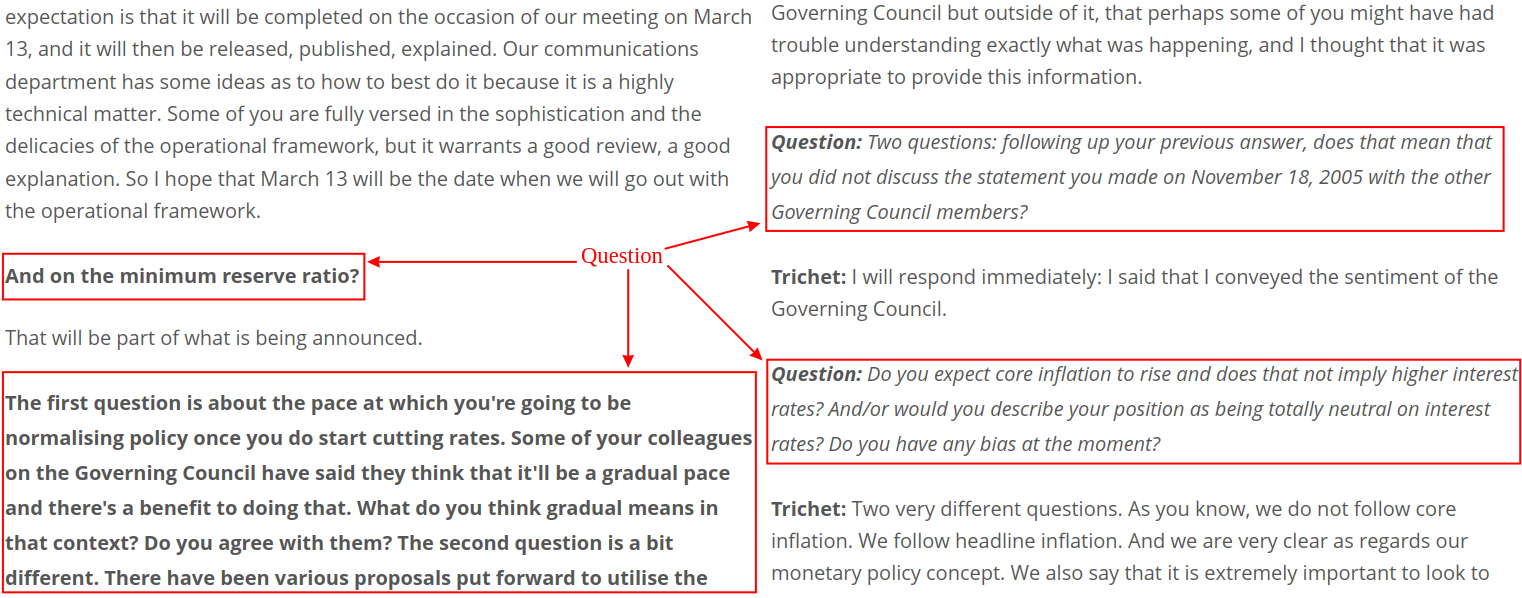
\includegraphics[width=1\linewidth]{images/data/qa_example_of_style.png}
    \caption[Evolution of formatting styles in ECB transcripts]{\centering Evolution of formatting styles in ECB transcripts. The~2005 transcript
        (right) utilizes explicit speaker labels, whereas the~2024 version (left) relies on font styling (bold/italic) to distinguish between
        speakers.}
    \label{fig:qa.styling}
\end{figure}

\section{Quantifying Central Bank Communications}
The~transition from qualitative narratives to quantitative market predictors requires a~systematic transformation of the~raw textual data. This stage of the~methodology is concerned with the~transformation of the~previous structured base dataset into a~more refined analytical collection. For this we use a~pipeline that reduces noise, considers limitations of models and adds metadata to the~text.

The~output of this pipeline is split into two specialized datasets that describe the~\gls{is} and \gls{qa} components. The~pipeline identifies themes through topic modelling. Moreover, it measures the~emotional tone of each observation via sentiment analysis. Unique identifiers are used to track the~original order of segments. This sustains the~chronological and contextual integrity of the~discourse. Binary classification is applied to the~\gls{qa} dataset to separate journalistic inquiries from official responses. This ensures the~analysis focuses on signals from\gls{ecb} officials.

\subsection{Text Segmentation and Contextual Windowing}

Further analysis requires strict rules, which enhance model behavior. By analyzing lengths and list of the~smallest paragraphs, we set the~minimum length of a~paragraph to $100$ characters. In this list, we observed redundant paragraphs, examples of which are provided in Table\ref{tab:redundant}. These passages are contextually sparse for transformers to identify the~sentiment or the~topic. Moreover, they do not hold valuable information for the~market audience.

\begin{table}[ht]
    \centering
    TODO doplniť reálne veci do tabuľky
    % v tabulke sa popis zvykne davat nad tabulku
    \caption{Illustrative examples of noisy paragraphs excluded from the~dataset.}
    %id tabulky
    \label{tab:redundant}
    % tu zacina samotna tabulka
    \begin{tabular}{@{}lr@{}}
        \toprule
        Paragraph content                                           & Character count \\ \midrule
        ``Thank you very much.''                                    & 21              \\
        ``I now leave the~floor to the~Vice-President.''            & 45              \\
        ``Question: Could you elaborate on the~inflation outlook?'' & 58              \\ \bottomrule
    \end{tabular}
\end{table}

Apart from this noise reduction, paragraph lengths often reach a~transformer’s token constraint, which is $512$ tokens per input for BERT-based models, including FinBERT and CentralBankRoBERTa. To address this, long paragraphs are processed into segments with an upper bound of $200$ words. This processing starts by partitioning passages into sentences using the~\textit{nltk.tokenize} library, which handles abbreviations and punctuation more robustly than simple splitting rules. The~preservation of full sentences is necessary for the~model's correct insight into the~context and syntactical structure of the~passage.

Our implementation follows an iterative approach where sentences are merged into a~segment until the~addition of the~next sentence would exceed the~maximum size. At that point, the~segment is closed, and a~new one is formed. Finally, for the~remaining text, we examine the~length of the~last segment of each paragraph. If this segment contains fewer than $30$ words, it is appended to the~preceding segment rather than being treated as an~independent input. This ensures that every segment processed by the~model contains sufficient semantic density, while the~combined length remains safely within the~transformer's token limitations.

Short paragraphs (that is, longer than $100$ characters but shorter than $30$ words) are maintained as independent segments. While shorter inputs may provide less context, their semantic integrity as independent statements or questions is considered more important for the~analysis than fulfilling a~word-count target. Finally, to ensure traceability, each segment retains the~metadata of its parent paragraph, including the~date, speaker identity, and section type (\gls{is} vs. \gls{qa}). This structure prevents the~``dilution'' of sentiment scores that occurs in excessively long text blocks and ensures that no segment is truncated. The~effectiveness of this segmentation and merging strategy is illustrated in Figure \ref{fig:distribution}, which compares the~word count distribution before and after the~transformation.

\begin{figure}[ht]
    \centering
    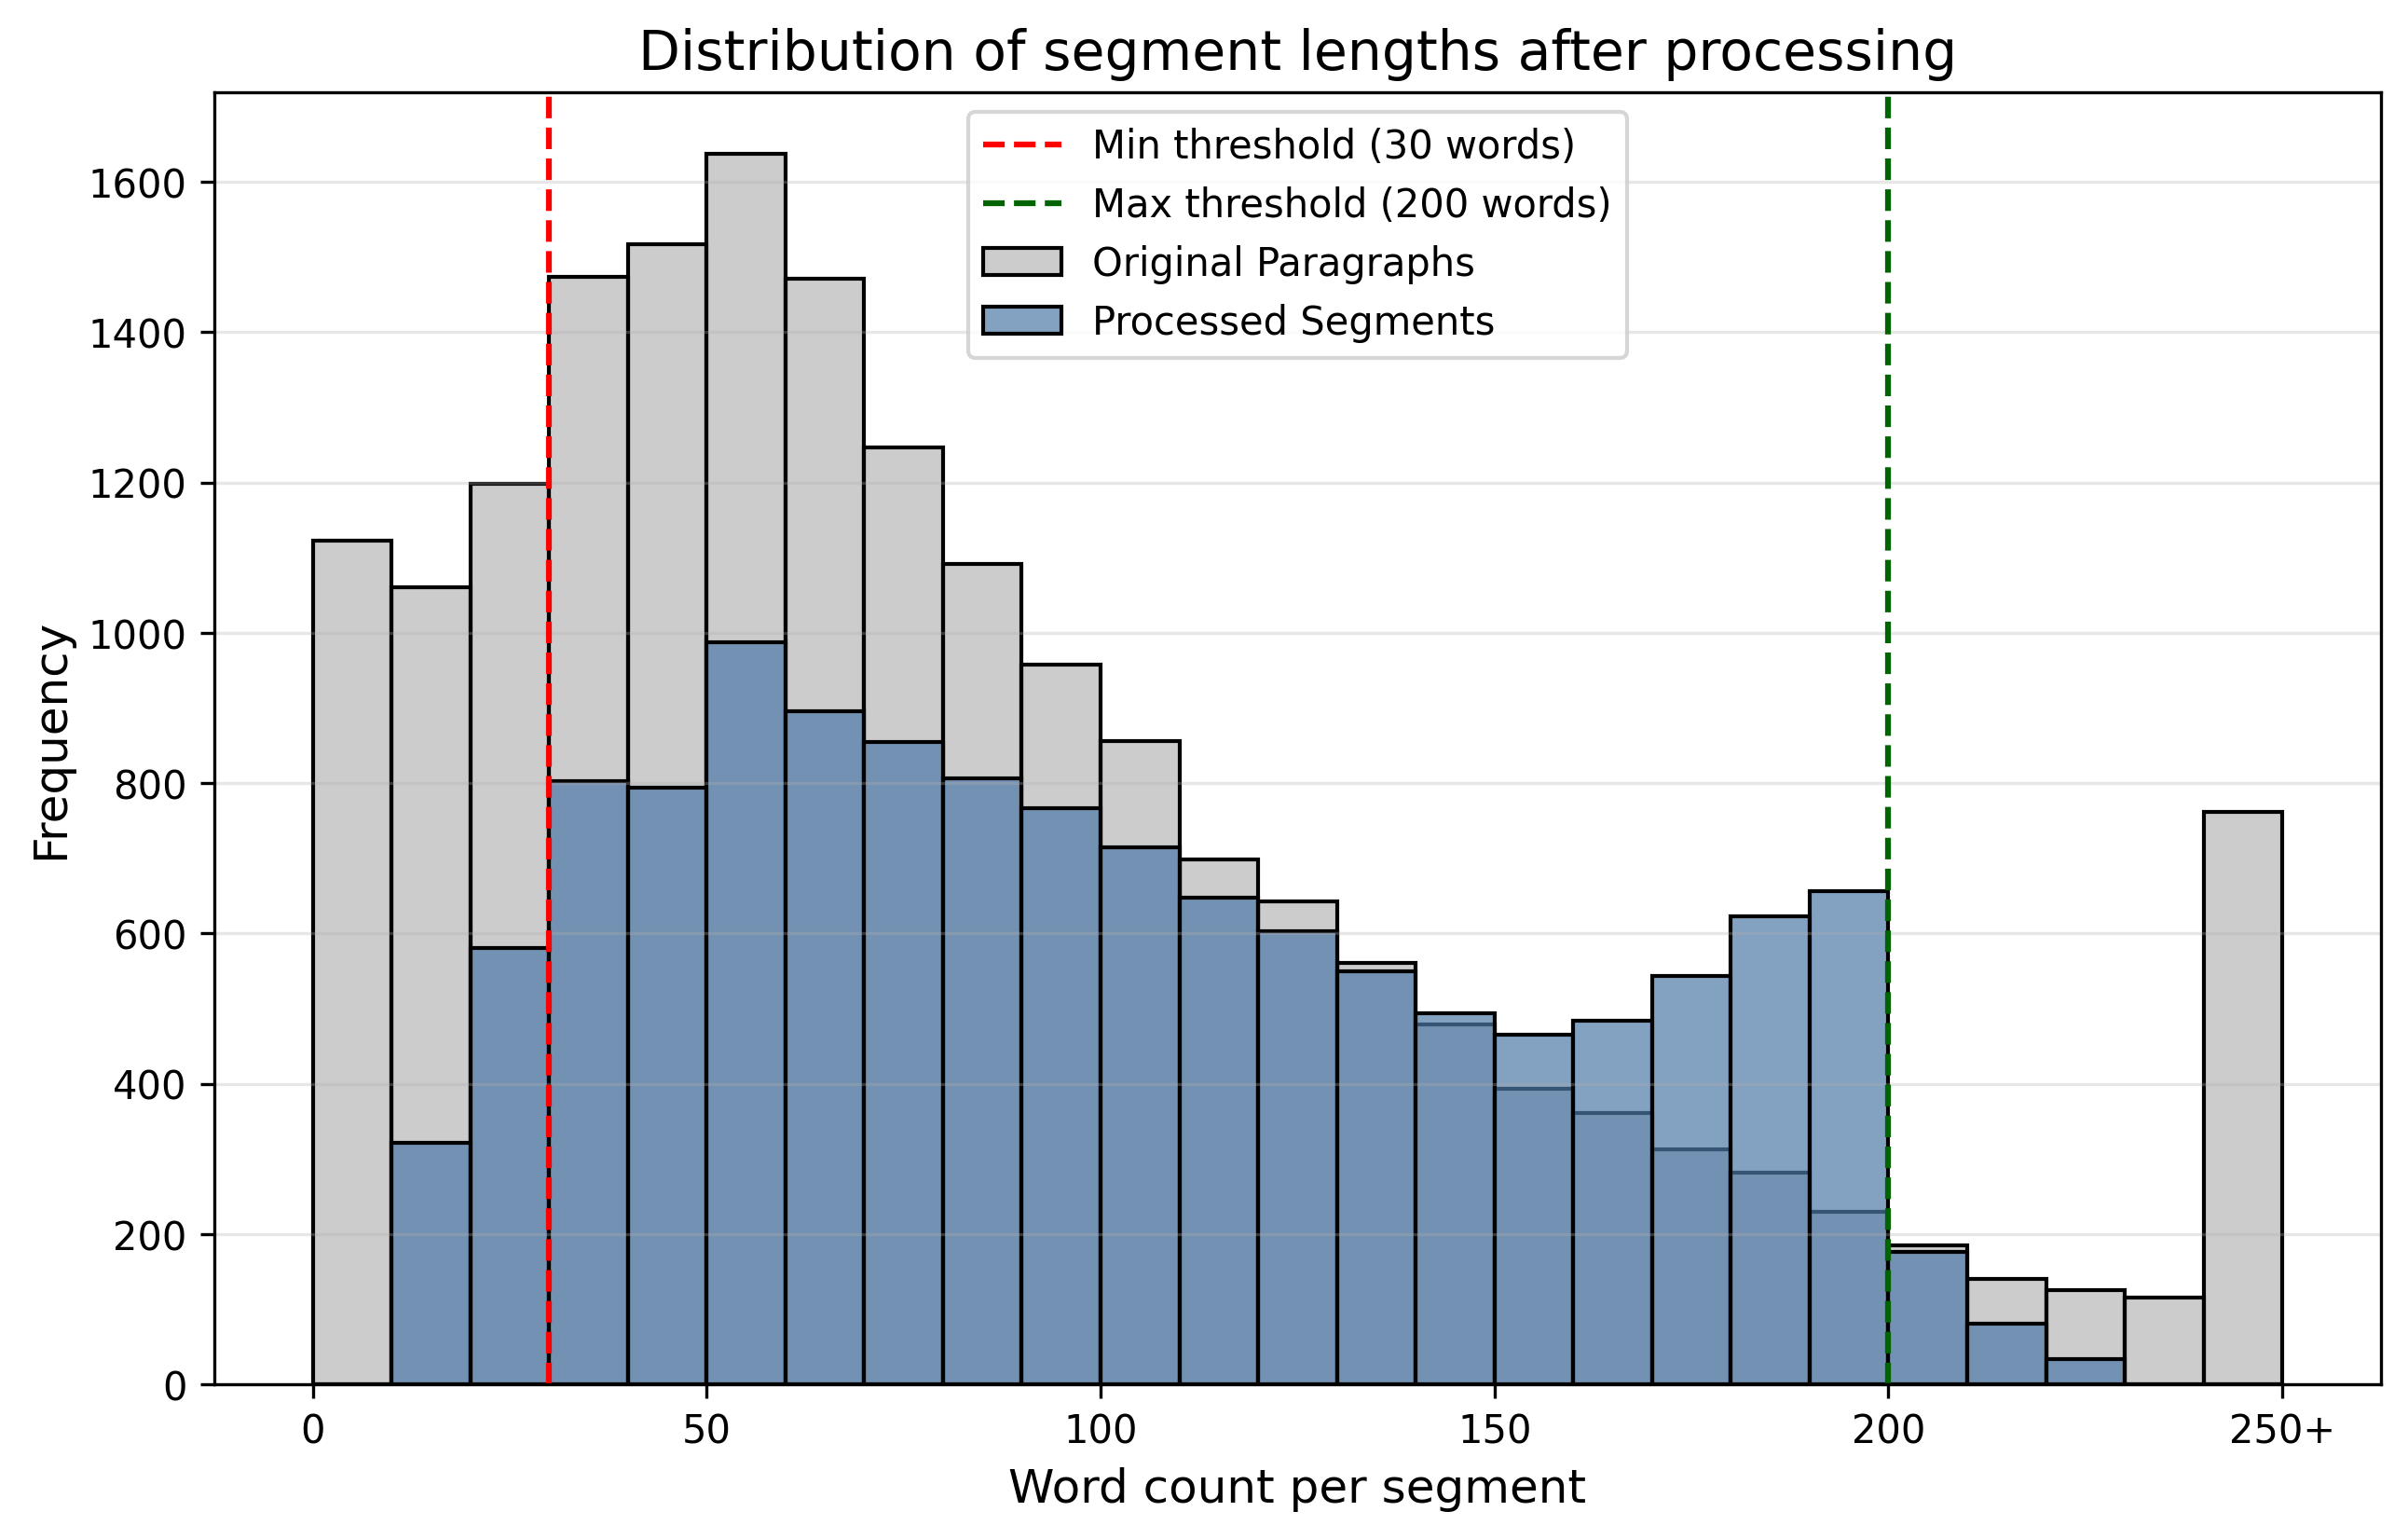
\includegraphics[width=1\linewidth]{images/data/segment_distribution.png}
    \caption[Impact of segmentation on text length distribution]{\centering Impact of segmentation on text length distribution. The~grey area
        represents original paragraphs with a~long tail of outliers, while the~blue area shows the~normalized segments adhering to the~$200$-word
        constraint.}
    \label{fig:distribution}
\end{figure}

\subsection{Zero-Shot Topic Classification}
While the~segments are now technically structured, they remain unlabelled raw text. To transform these strings into meaningful predictors, we must categorize them based on their thematic content. We considered several approaches to this task. Traditional Dictionary-based (Bag-of-Words) methods were dismissed due to their inability to capture context, such as negations or complex sentence patterns. Furthermore, training a~custom Topic modelling transformer on annotated data was not feasible given the~project’s time constraints and the~lack of a~pre-labelled domain-specific dataset.

Consequently, we decided to implement Zero-Shot Classification. This approach allows for the~classification of text into prescribed categories without requiring  explicit training on those specific labels. After reviewing current state-of-the-art models, we selected the~\textit{facebook/bart-large-mnli} model. This model is particularly suitable for our use case. Thus, it is pre-trained on Natural Language Inference (NLI) tasks. Further, it enables treating thematic labels as hypotheses to be tested against the~text segments.

We also started with a~list of ten detailed topics. This turned out to be a~mistake, because the~model suffered from a~sort of decision paralysis (much like a~human struggling to choose from a~massive menu). It became indecisive and ended up dumping almost everything into a~broad ``Risk Assessment'' category. To fix this, we radically simplified the~taxonomy to four core themes and replaced the~short titles with descriptive hypothesis strings. By narrowing the~choices and enriching the~context of each label, we forced the~model to be more certain. The~final set of labels and their descriptive strings are detailed in Table \ref{tab:labels}.
\begin{table}[ht]
    \centering
    \caption{Thematic labels and descriptive strings for Zero-Shot Classification}
    \label{tab:labels}
    \begin{tabular}{@{}lp{8cm}@{}}
        \toprule
        \textbf{Category}                & \textbf{Model Input (Label String)}                                            \\ \midrule
        Monetary Policy                  & ``inflation, price stability, interest rate decisions, monetary policy stance,
        financing conditions, bank lending, and market interest rates''                                                   \\ \addlinespace
        Economic Performance             & ``economic growth, GDP outlook, unemployment, labor market developments,
        macroeconomic risks, demand, consumption, and investment''                                                        \\ \addlinespace
        Fiscal             \& Structural & ``government budgets, national debt, public spending, and structural reforms'' \\ \addlinespace
        Other / Noise                    & ``general greetings, purely political questions, unrelated remarks, climate
        change, or personal comments (excluding macroeconomic impacts)''                                                  \\ \bottomrule
    \end{tabular}
\end{table}

The~``Other'' category is our final filter. It catches thematic noise. This noise includes politeness and procedural talk that doesn't actually move markets. By isolating these, we can later test if stripping away the~fluff actually sharpens our sentiment-based market predictions.

\subsection{Multi-Model Sentiment Extraction}
Once the~segments are labeled, the~next step involves extracting the~actual emotional tone (the~sentiment) from the~text. To ensure a~robust assessment, this research adopts a~parallel approach using two distinct architectures. This approach accounts for the~varying linguistic nuances captured by different model pre-training objectives. Therefore, we use a~two models paralleling approach (FinBERT and CentralBankRoBERTa) to evaluate every chunk in both the~\gls{is} and \gls{qa} datasets.

The~choice of these two models is intentional. FinBERT is the~industry standard for general financial text, while CentralBankRoBERTa is specifically tuned to recognize the~unique language of central bankers. It understands categories like ``Hawkish'' (signaling tighter policy) and ``Dovish'' (signaling looser policy). These categories are far more useful for our analysis than simple positive or negative labels. For both models, the~net sentiment score for each segment is calculated following the~methodology established in Equation \ref{eq:sentiment}.

In this setup, neutral sentences are assigned a~value of zero. This represents a~methodological choice, because neutral segments effectively act as a~``diluent'' that reduces the~overall intensity of the~signal. If a~press conference is filled with neutral filler text, the~final score should naturally gravitate toward zero.

Instead of just looking at the~average sentiment, we calculate a~whole suite of metrics for the~entire \gls{is} and \gls{qa} components separately. These include the~mean, minimum, maximum, and the~standard deviation of the~scores. Our logic is that financial markets don't always react to the~average tone. Sometimes, a~single extreme statement (the~maximum or minimum) can move the~needle more than the~rest of the~speech combined. The~standard deviation also helps us see if the~ECB's message was consistent or if it fluctuated wildly during the~session.

Finally, we produce two distinct outputs for our empirical model. The~first is a~``general'' sentiment, which looks at the~text as a~whole without any filters. The~second is a~``labeled'' sentiment, where we weight the~scores based on the~topics identified in the~previous step. This allows us to test a~key hypothesis: does the~market care more about the~sentiment regarding inflation than, for example, the~sentiment regarding general economic growth?

To demonstrate how these models process the~ECB's language in practice, we provide a~few illustrative examples in Table \ref{tab:sentiment_examples}. These segments show how FinBERT and CentralBankRoBERTa assign different weights to the~same sentence, underscoring the necessity of a~multi-model evaluation. For instance, a~sentence about stagnant growth might be seen as purely ``Negative'' by FinBERT, while CentralBankRoBERTa might interpret it as a~``Dovish'' signal for future interest rates.

\begin{table}[ht]
    \centering
    \caption{Illustrative comparison of net sentiment scores between models}
    \label{tab:sentiment_examples}
    \begin{tabular}{@{}lp{7cm}cc@{}}
        \toprule
        \textbf{Source} & \textbf{Text Segment (Sample)}                             & \textbf{FinBERT} & \textbf{RoBERTa} \\ \midrule
        IS              & ``Inflation is expected to remain too high for too long.'' & 0.12             & 0.88             \\ \addlinespace
        \gls{qa}        & ``Economic activity has stagnated in recent quarters.''    & -0.75            & -0.42            \\ \addlinespace
        IS              & ``We will continue to follow a~data-dependent approach.''  & 0.00             & 0.05             \\ \bottomrule
    \end{tabular}
\end{table}

\section{Relational Database Integration}
The~final stage of the~text processing pipeline involves migrating the~segments and their  metadata from temporary flat files into a~relational database. To manage the~outputs of the~\gls{nlp} models and ensure data integrity, we designed a~custom \texttt{SQLite} schema. This architecture is essential for maintaining the~hierarchical relationship between the~original monetary policy events and the~granular textual units produced during the~windowing phase.

The~core of the~system is the~\texttt{chunks} table, which serves as the~primary link between the~raw text and its analytical features. Each segment is tagged with a~boolean flag to distinguish between questions and responses, ensuring that the~final policy signal remains untainted by external sentiment. Furthermore, the~database stores the~segments at multiple granularities, including the~sentence-level baseline and larger contextual blocks. This decoupling of text from model outputs allows for simultaneous storage of scores from diverse architectures, such as \textit{FinBERT} and \textit{CentralBankRoBERTa}, in the~\texttt{sentiments} table.

By organizing the~data relationally, we eliminate the~need for redundant text parsing during the~econometric analysis. The~thematic distributions from the~zero-shot classifier are stored in the~\texttt{topics} table, allowing for complex SQL queries that can instantly aggregate sentiment across specific macroeconomic categories. This database, summarized in Table \ref{tab:db_schema}, provides the~necessary stability for the~subsequent modeling of interactions between central bank discourse and financial market variables.

\begin{table}[ht]
    \centering
    \caption{Relational Database Schema Overview}
    \label{tab:db_schema}
    \begin{tabularx}{\textwidth}{@{}ll >{\raggedright\arraybackslash}X @{}}
        \toprule
        \textbf{Table Name} & \textbf{Primary Key} & \textbf{Description and Relational Role} \\ \midrule
        \texttt{statements} & \textit{rowid} & Master log of \gls{mps} events, chronological metadata, and source URLs. \\
        \texttt{chunks}     & \textit{chunk\_rowid} & The central entity storing segmented text, speaker flags, and part identifiers. \\
        \texttt{sentiment\_models} & \textit{model\_rowid} & Registry of \gls{nlp} architectures (e.g., FinBERT, RoBERTa) used for sentiment extraction. \\
        \texttt{sentiments} & \textit{composite} & Maps specific chunks to raw scores, linked to \texttt{sentiment\_models} for multi-model comparison. \\
        \texttt{topic\_labels} & \textit{name, version} & Reference table for the macroeconomic taxonomy and descriptive hypothesis strings. \\
        \texttt{topics}     & \textit{chunk\_rowid, label\_rowid} & Stores probability scores, linking textual segments to defined expert themes. \\ \bottomrule
    \end{tabularx}
\end{table}

\section{Financial Market Data}
To evaluate the~information value of central bank discourse, we utilize a~comprehensive set of financial indicators that capture both official policy decisions and high-frequency market reactions. The~primary source for market expectations is the~\textit{Euro Area Monetary Policy Event-Study Database} (EA-MPD), as compiled by \cite{altavilla2019measuring}. This dataset provides changes in \gls{ois} rates across multiple maturities, from 1-month to 10-years, measured within a~narrow window around the~press conference. These high-frequency changes are essential for isolating the~``surprise'' component of the~communication, as they filter out other macroeconomic news occurring on the~same day.

Complementing the~market-based expectations, we incorporate official policy rates and model-based proxies for the~\gls{ecb}'s stance. The~Main Refinancing Operations (\gls{mro}) rate represents the~explicit signal of the~policy target. However, to account for periods where interest rates are constrained by the~Zero Lower Bound, we include the~Wu-Xia Shadow Rate as a~proxy for the~unconstrained monetary conditions. Furthermore, we utilize the~first principal component ($PC1$) of structural shocks, which aggregates the~policy surprise across the~entire yield curve into a~single, robust target variable. These variables, sourced from the~\gls{ecb} Money Market archives and structural decomposition models, provide the~quantitative benchmark against which the~textual sentiment is assessed.

\section{Empirical Model Specification}


\chapter{Results}
In this chapter we will talk about evaluations and results of our thesis.
\section{Evolution of ECB Sentiment}
\section{Sentiment Differences: Statement vs. Q\&A}
\section{Regression Analysis Results}
\chapter{Discussion}
\label{ch:discussion}
In this chapter we will leave a room for questions and answers.
\section{Implications for Policy Makers and Markets}


% \input chapter.tex

\chapter*{Conclusion} % chapter* je necislovana kapitola
\addcontentsline{toc}{chapter}{Conclusion} % rucne pridanie do obsahu
\markboth{Conclusion}{Conclusion} % vyriesenie hlaviciek

This thesis has examined how machine-learning analysis of the textual record of \gls{ecb} press conferences quantifies, structures, and ultimately prices the information that the central bank communicates to financial markets. Working with a custom corpus of $289$ press conferences from June~1998 to October~2024, and a pipeline that separates the prepared \gls{is} from the spontaneous \gls{qa} and, within the \gls{qa}, journalists' questions from the President's answers, the empirical chapters delivered four findings.

First, FinBERT and CentralBankRoBERTa produce internally coherent series whose turning points align with the canonical episodes of the euro-area cycle: the October~2008 rate cut, Draghi's 2012 ``Whatever it takes'' speech, the 2015 \gls{qe} launch, the 2020 pandemic emergency, and the 2022 hiking lift-off. Two encoder families trained on different corpora agree on the sign of the signal, which is the minimum bar for treating the textual measure as more than a model artefact.

Second, the \gls{is} and the \gls{qa} are structurally different communicative acts. The \gls{is} traces a coherent three-act narrative arc---moderate opening, risk-catalogue trough, hawkish policy-decision close---with a within-conference swing of roughly $0.4$ FinBERT units, while the \gls{qa} is essentially flat as a function of relative position. Within the \gls{qa}, journalist questions are systematically more dovish than the \gls{ecb}'s answers, by an average of $0.29$ on the CentralBankRoBERTa scale, and this gap is stable across the Pre-\gls{zlb}, \gls{zlb}, and hiking regimes. Without separating the two voices, the press corps' affective tone would contaminate the policy signal by approximately $0.3$ units---an order of magnitude that is large relative to the policy-relevant variation. The structural decomposition of the press conference is therefore not an optional refinement but a methodological prerequisite for any sentiment-based study of central-bank communication, and is one of the principal departures of this thesis from earlier studies that treat the press conference as a single document.

Third, sentiment leads the \gls{ecb}'s policy decisions rather than tracking them coincidentally. The event-study window of $\pm 6$ meetings shows a hawkish profile fully established up to six meetings before an actual hike in the pre-\gls{zlb} period and a symmetric telegraphing of both hikes and cuts in the post-pandemic cycle. The lag-correlation analysis identifies a peak between the FinBERT overall mean and the \gls{mro} change at a lag of four meetings ($r = 0.551$ on changed meetings).

Fourth, the textual signal carries incremental predictive content for the direction of the next \gls{ecb} rate decision. Four classifiers were compared on a three-class target: a rate-history baseline (M1), a sentiment-only logit (M2), an augmented logit (M3), and a Random Forest on the same feature set (M4). The cross-validated AUC ordering is strict: $0.682 < 0.694 < 0.705 < 0.763$. The M2-versus-M1 increment establishes that the text adds directional information beyond the rate history alone; the M4-versus-M3 increment of $+0.058$ shows that an economically meaningful portion of that information is carried by non-linear interactions which the logistic specification cannot capture. The textual record and the rate history are complementary rather than redundant.

Four extensions are particularly natural. First, the affective-sentiment layer should be replaced with a dedicated \emph{stance classifier} that assigns the operationally meaningful hawkish/dovish/neutral label rather than positive/negative tone; the \gls{zlb}-era flatness of the present series is a direct artefact of the sentiment--stance mismatch, and a stance-aware classifier would close it. The gated state-of-the-art models of Shah et al.\ \cite{shah2023trillion, shah2025wcb} are the most direct route, but a custom classifier fine-tuned on a manually annotated \gls{ecb} corpus is feasible at modest annotation cost. Second, large language models such as GPT-4o or Claude can serve as zero-shot stance annotators at near-human quality, providing a silver-standard label set for distillation into a smaller deployable encoder; reproducibility requires fixing temperature and logging the model version. Third, the daily \gls{ois} reaction used here can be replaced by the intraday windows of the Euro Area Monetary Policy Event-Study Database \cite{altavilla2019measuring}, separating the $14{:}15$~CET press-release window from the $14{:}45$--$15{:}15$~CET press-conference window; this directly tests the hypothesis that the \gls{qa} signal is the slower-incorporating of the two. Fourth, and most importantly from the policy perspective, the pipeline can be replicated on the press conferences of the Federal Reserve and the Bank of England under identical chunking, classification, and aggregation rules. This cross-bank replication is the planned next step in the collaboration with the Národná banka Slovenska and forms the empirical core of the envisaged co-authored publication: the cross-bank profile of communication asymmetry will directly inform the conditions under which a small open economy facing the euro area should treat \gls{ecb} sentiment as a leading indicator versus a contemporaneous signal.

The qualitative record of monetary policy can be read systematically, separated cleanly into its prepared and spontaneous components, and converted into a structured time series with measurable predictive value for the price of money. The framework developed in this thesis is one step in that programme; the limitations identified along the way describe extensions of scope rather than barriers to the central conclusion.



% \input zaver.tex

% -------------------
% --- Bibliografia
% -------------------


\newpage	

\backmatter

\thispagestyle{empty}
\clearpage

\bibliographystyle{plain}
\bibliography{literatura} 
\addcontentsline{toc}{chapter}{References}


% -------------------
%--- Prilohy---
% -------------------

%Nepovinná časť prílohy obsahuje materiály, ktoré neboli zaradené priamo  do textu. Každá príloha sa začína na novej strane.
%Zoznam príloh je súčasťou obsahu.
%
% \input appendixA-en.tex

% \input appendixB-en.tex

\end{document}






